\section{Anhang}
\nopagebreak
\begin{table}[h]
\scriptsize
\centering
\begin{tabular}{rllll}
t & x-Pos. $m_1$ & y-Pos $m_1$ & x-Pos. $m_2$ & y-Pos. $m_2$ \\
\toprule
\end{tabular}
\normalsize
\caption{Verlauf der Position der beiden Massen über die Zeit des Versuchs. Dabei wird t in s und die Position in m gemessen.}
\label{xy-table}
\end{table}


\begin{figure}
\centering
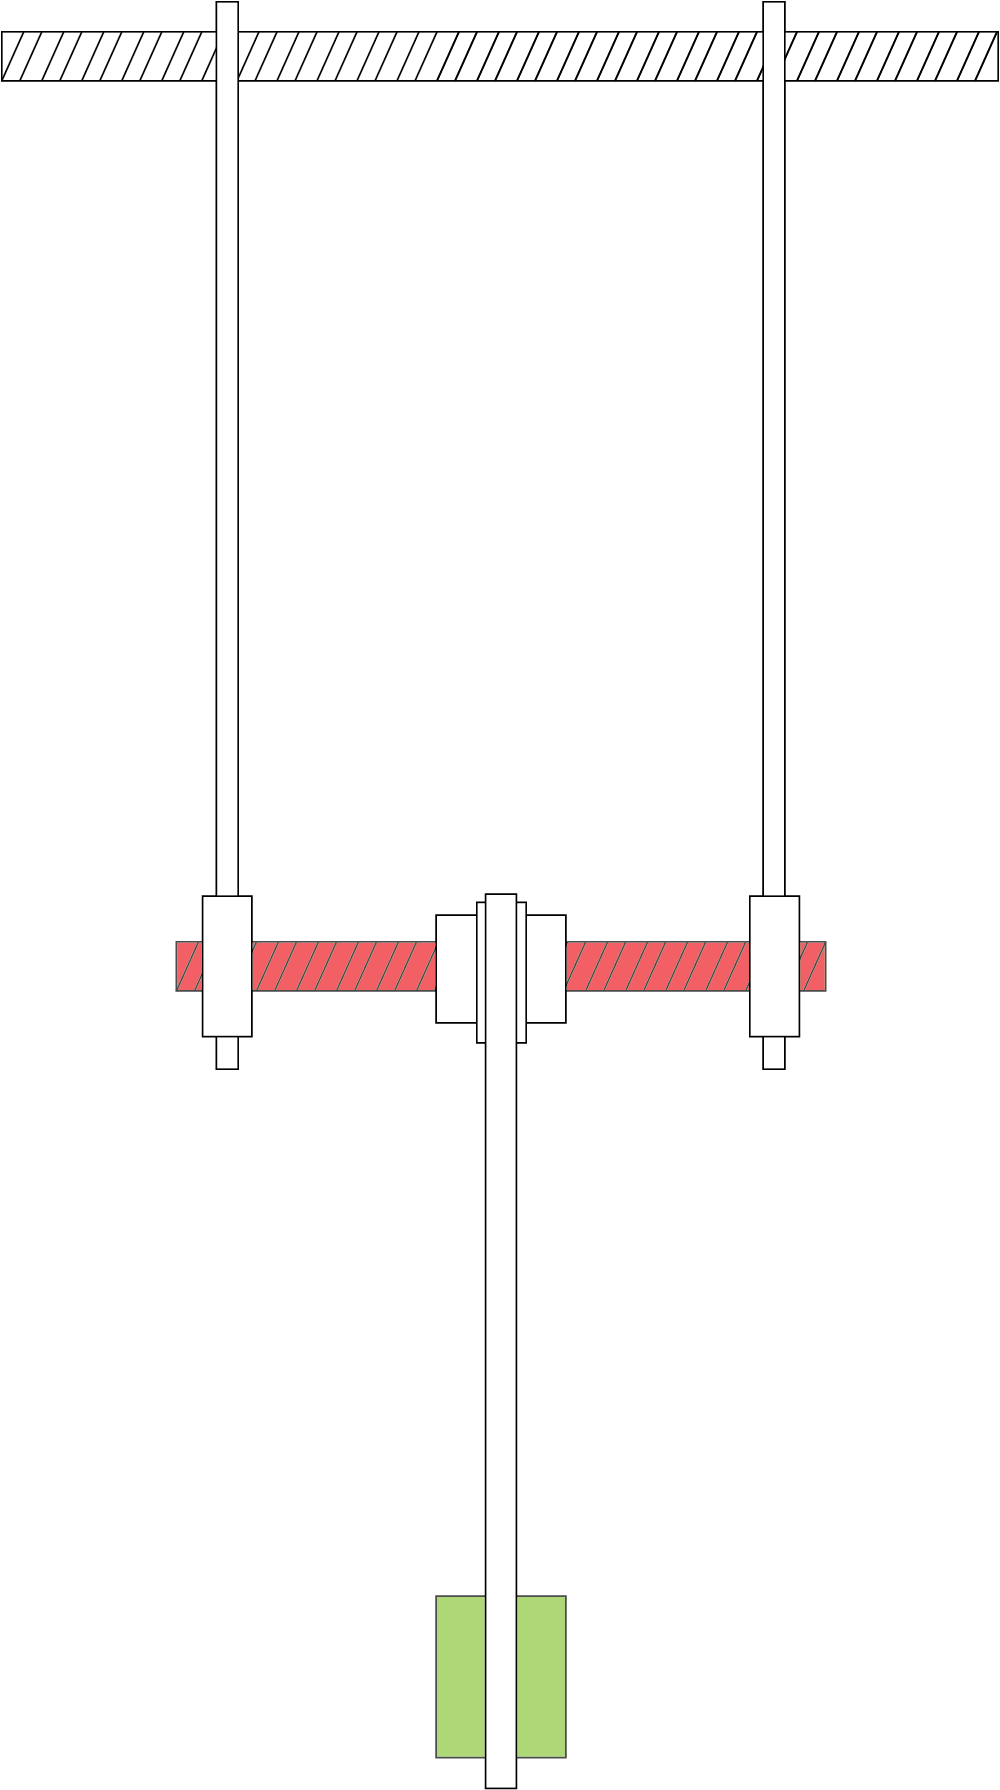
\includegraphics[width=.6\textwidth]{images/pendel-skizze.png}
\label{pic:skizze_versuchsaufbau}
\end{figure}